\documentclass[usegeometry=true]{scrartcl}
\usepackage[ngerman]{babel}
\usepackage[T1]{fontenc}
\usepackage{lmodern}
\usepackage[utf8]{inputenc}
\usepackage{hyperref}
\usepackage{amssymb}
% Dimensionen bitte nicht ändern. 
\usepackage[left=2cm, right=2cm, top=2cm, bottom=2cm, bindingoffset=1cm, includeheadfoot]{geometry}
%Zeilenabstand bitte nicht ändern
\usepackage[onehalfspacing]{setspace}


% --- Abkürzungsverzeichnis ---
\usepackage[nohyperlinks, 
withpage, 
smaller,
footnote
]{acronym}



% --- Grafiken ---
\usepackage{graphicx}
\usepackage{subfig}



\usepackage[backend=biber,style=numeric,]{biblatex}\addbibresource{Visualisierung.bib}

\begin{document}
\pagenumbering{Roman}
% ----------------------------------------------------------------------------
\subject{Projektbericht zum Modul Information Retrieval und Visualisierung Sommersemester 2021}
\title{Visualisierung von Daten des Videospiels Fifa 21}
%\subtitle{Untertitel}% optional
\author{Johannes Lange}% obligatorisch
%\date{10.9.2021}
\maketitle% verwendet die zuvor gemachte Angaben zur Gestaltung eines Titels
%
\newpage
%----------------------------------------------------------------------------
% Inhaltsverzeichnis:
\tableofcontents
\newpage

% Abbildungsverzeichnis
\clearpage
\listoffigures

% Abkürzungsverzeichnis:
\section*{Abkürzungsverzeichnis}\label{AV}
	\addcontentsline{toc}{section}{Abkürzungsverzeichnis}
	\begin{acronym}
	\acro{FUT}[FUT]{Fifa Ultimate Team}
	\end{acronym}
\newpage
% ----------------------------------------------------------------------------
% Gliederung und Text:
\pagenumbering{arabic}
\section{Einleitung}

% -Zu Parallel Koordinaten on Hover inklusive der verglichenen Werte hinzufügen
% -Aggregationsfunktion möglicherweise entfernen, überprüfen ob der Code deutlich schneller läuft
% -Torhüter herausfiltern, da diese keine Werte haben
% -Filter Funktion in parallelen Koordinaten und Scatterplot erweitern
%Tipps zu Latex und Koma-Script für Hausarbeiten sind im \href{http://mirrors.ctan.org/info/latex-refsheet/LaTeX_RefSheet.pdf}{LaTeX Reference Sheet for a thesis with KOMA-Script} von Marion Lammarsch und Elke Schubert zusammengefasst. 
%Der Bericht fällt in die Kategorie von InfoVis-Paper, die Tamara Munzner Design Study nennt \cite{Munzner2008}: In der Einleitung sollen sie zuerst das Zielproblem beschrieben. Daraus sollen sie Fragestellungen motivieren, die mittels Techniken der Informationsvisualisierung beantwortet werden können. 

%\textbf{Tamara Munzner angucken}\\
%\textbf{Zielprobelm formulieren und daraus Fragestellung schreiben -> Wie können diese mittels Visualisierung beantwortet werden}


Die Visualisierung von Daten nimmt mit Hinblick auf Big Data und damit immer unübersichtlicheren Datengrundlagen an Bedeutung zu. Um aus großen Mengen von Daten neue Informationen zu gewinnen reicht es nicht aus die Daten direkt zu analysieren. Durch die Anwendung der richtigen Visualisierungstechniken können neue Informationen gewonnen werden. In diesem Bericht geht es um die Visualisierung von Daten aus dem Computerspiel Fifa 21. Da sich diese Daten allerdings auf tatsächliche Fussballer beziehen besteht die Hoffnung mittels Visualisierung dieser Daten Rückschlüsse auf die Sportler selbst schließen zu können.
So könnten Erkenntnisse aus den Daten deutlich wertvoller sein als zuerst vermutet.\\
Der gegebene Datensatz ist äußerst umfangreich, zu über 16000 Sportlern sind jeweils 107 Variablen festgehalten. Diese reichen von \textit{Name} über \textit{Verein} bis hin zu \textit{Schusskraft} eines Spielers. Da nicht alle Eigenschaften eines Fussballers konkret festgehalten werden können, sind einige der Werte geschätzt. Da aus diesem Grund wie oben beschrieben nicht sicher auf die tatsächlichen Spieler zurückgeschlossen werden kann, bietet sich eine Analyse der Daten bezüglich der Nähe zur Realität an. Doch selbst wenn die Daten nicht zu neuen Erkenntnissen bezüglich der realen Sportler führen können sich für Spieler des Videospiels neue Erkenntnisse ergeben. 


\subsection{Anwendungshintergrund}
%Sie müssen genug Hintergrund bereitstellen, so dass die Lesenden sich ein Urteil bilden können, ob ihre Lösung funktioniert. Sie sollen die Lesenden jedoch nicht mit Anwendungsdetails so überschütten, dass der Fokus auf die Fragen zur Informationsvisualisierung untergehen. 
\textbf{Was sind die Daten, sind die Visualisierungslösungen angebracht, möglicherweise auf einzelne Variablen eingehen}\cite{Munzner2008}

Im folgenden werden die drei verwendeten Visualisierungstechniken kurz vorgstellt und erklärt.
Bei der ersten Visualisierungstechnik handelt es sich um einen Scatterplot. Mit diesem lassen sich Zusammenhänge zwischen zwei verschiedenen Attributen der Fussballer genauer untersuchen. So kann bspw. gezeigt werden ob sich das Alter eines Fussballers auf seine Bewertung im Spiel auswirkt.
Die zweite Visualisierungstechnik ist die der parallelen Koordinaten. Diese eignet sich auf Grund ihrer Beschaffenheit dazu mehrdimensionale Daten zu untersuchen. In diesem Fall wurde sich für parallele Koordinaten mit vier verschiedenen Attributen entschieden um eine gewisse Überischtlichkeit zu wahren.

Die Frage, welche sich bei diesen Daten stellt ist, welchen Nutzen sie außerhalb eines Videospiels haben. Deswegen ist mein Ansatz zu vergleichen wie genau diese Daten die Wirklichkeit widerspiegeln. Ein Beispiel dafür könnte sein ob sich das Rating eines Spielers mit der körperlichen Entwicklung eines Spielers bewegt. Sollte dies zutreffen  müssten Spieler im Alter ihres physischen Peaks das höchste Rating haben. 
\subsection{Zielgruppen}
%Beschreiben sie die Personengruppe oder Personengruppen, die das von ihnen benannte Anwendungsproblem lösen möchte. Auf welches Vorwissen können sie in dieser Gruppen von Anwenderinnen aufbauen? Welche Informations"-bedürf"-nisse werden durch die Visualisierungen adressiert?
Da es sich bei den Daten um die eines Videospiels handelt ist davon auszugehen, dass eine der Zielgruppen der Daten Spieler des Videospiels sind. Diese würde ich weiterhin in die des Spielmodus \textit{Karriere} und die des Spielmodus \textit{Fifa Ultimate Team  FUT} unterteilen.\\

Spieler des Karrieremodus spielen das Spiel als Manager eines Vereins indem die Entwicklung von jungen Spielern wichtig ist und vor allem der Vergleich von Variablen wie Gehalt, Alter, Rating oder Potential relevant ist. In diesem Fall bietet sich eine Darstellung per Scatterplot an, da sich so schnell die aussichtsreichsten Fussballer erkennen lassen. Da der Karrieremodus nicht Online gespielt wird und die Schwierigkeit manuell festgelegt werden kann, ist davon auszugehen, dass das Vorwissen der Gruppe stark schwankt. Während einige Spieler bereits viel Wissen und sehr genaue Informationen benötigen, brauchen andere erst einmal Grundwissen bezüglich der Spieler.

Spieler des FUT Modus sammeln die Fussballer wie in einer Art Sammelkarten Spiel. Mit den Karten der Fussballer kann dann Online gegen andere Spieler angetreten werden. Dabei sind vor die aktuellen Werte der Spieler von Relevanz, da sich diese nicht durch Training oder ähnliches ändern lassen. Weil dieser Modus sehr kompetetiv ist kann ein Fussballer bereits durch einen schlechten Wert in einer Kategorie für Spieler unbrauchbar werden. Dadurch, dass \textit{FUT} zu den Onlinespielen gehört in denen viele Spieler sich durch \textit{Min-Maxing}\cite{noauthor_min-maxing_2014} einen Vorteil verschaffen wollen ist von einem hohen Vorwissen der Anwender der Visualisierung auszugehen.  




\textbf{Fifa 19 Spieler -> Viel Vorwissen, Fussball Fan -> recht viel Vorwissen, Sportinteressent -> Kaum Vorwissen}

Zielgruppen für Scatterplot:\\
Parallele Koordinaten:\\
Baumdiagramm: Hier lässt sich erkennen welche Sportliga Europas im Durchschnitt die besten Spieler hat. Deswegen ist dies für X interessant.\\
Mögliche Zielgruppen: Videospieler, Teilnehmer einer Fantasy Fußball Liga
\subsection{Überblick und Beiträge}
%In diesem Abschnitt geben sie einen kurzen Überblick über die Daten und verwendeten Visualisierungen. Dann benennen sie die Beiträge ihres Projekts. Diese Beiträge müssen sie in den hinteren Teilen des Berichts genauer ausführen und belegen.

%\textbf{Sehr kurze Beschreibung der Daten, der Drei Techniken und Beiträge des Projekts(Mehrwert der Visualisierungstechniken)} 


Bei den Daten handelt es sich um einen Datensatz des Fussball Videospiels Fifa 19 dieser enthält Daten zu über 18000 Fussballern. In diesen enthalten sind neben Variablen wie Name, Verein und Alter auch ein ungefähr nach der Qualität des Fussballers festgelegtes Rating sowie Bewertungen seiner fussballerischen Fähigkeiten (Schießen, Passen, Dribbling, Verteidigen, Geschwindigkeit, Physis, etc.)\\

Die erste verwendete Visualisierungstechnik ist der Scatterplot, dieser ist gut dazu geeignet zwei Variablen der Fussballer zu vergleichen. Bspw. könnte untersucht werden ob ein Fussballer entsprechend seines Könnens (Rating) verdient (Wage). \\

Bei der zweiten verwendeten Visualisierungstechnik handelt es sich um Parallele Koordinaten. Diese, im Vergleich zum Scatterplot, etwas fortgeschrittene Technik eignet sich um mehr als zwei Werte miteinander zu vergleichen. Ihr Einsatz bietet sich daher an um Werte eines Fussballers in den Attributen: Schießen, Passen, Dribbling, Verteidigen, Geschwindigkeit oder Physis miteinander zu vergleichen und dies vorher nach der Position des Fussballers zu Filtern um zu untersuchen ob sich ein Spieler anhand seiner Attribute dafür eignet auf dieser Position zu spielen. (Bsp. ein Stürmer benötigt vor allem Geschwindigkeit, Schießen und Dribbling, ein Verteidiger hingegen Verteidigen, Physis und Geschwindigkeit).\\

Die dritte Visualisierungstechnik ist die Darstellung als Baumdiagramm. durch sie werden Spieler ihren Teams und diese ihren jeweiligen Ligen zugeordnet.



Als dritte und letzte Technik habe ich die Baumdarstellung ausgewählt um sichtbar zu machen welche Fussballliga Europas im Durchschnitt die besten Spieler hat. Deswegen ist dies für X interessant.\\

\section{Daten}
%Beschreiben Sie vorhandenen Daten. Gehen sie kritisch darauf ein, in wie weit sich die Daten für die Bearbeitung der Fragestellungen und dem Erreichen von Lösungen für die oben beschriebene Zielgruppen eignen. Haben sie die Daten sinnvoll mit weiteren Datenquellen ergänzt? Wenn ja, wie?

\textbf{Beschreibung der gegebenen Daten, Sind sie zur Beantwortung der Fragestellungen geeignet? Welche zusätzlichen Daten wurden genutzt} 

Grundsätzlich eignen sich die Daten gut um die gewünschten Fragestellungen beantworten zu können, jedoch enthält der Grunddatensatz einige Felder, die für die Visualisierung nicht nötig sind, deswegen wurde der Datensatz in der Vorvorarbeitung noch verkleinert (Siehe \ref{Datenvorverarbeitung} auf Seite \pageref{Datenvorverarbeitung}). Außerdem ist der Datensatz sehr groß, was gerade bei den parallelen Koordinaten zu Problemen führen kann wenn der ganze Datensatz angezeigt wird, deswegen wurde sich bei den parallelen Koordinaten dazu entschieden nach zusätzlichen Dimensionen wie Nationalität zu Filtern um dies so übersichtlicher zu gestalten. Da Datenwerte wie Größe, Alter und Rating der Spieler diskret sind wurde sich dazu entschieden im Scatterplot die Anzahl an Spielern welche in diesem Punkt enthalten sind auszugeben. Weiterhin wurde die Opazität der Punkte verringert, da so zu sehen ist an welchen Stellen sich mehrere Spieler überlagern. 
\subsection{Technische Bereitstellung der Daten}
%Wie sind die Daten zugänglich? Welche Formate werden genutzt. Gibt es Besonderheiten beim Lesen der Formate?
Die Daten sind in einem privaten Github gehostet\footnote{\url{https://github.com/JohannesLange/Visualisierung_FIFA19/tree/master}}. Dort liegen die Daten der drei Visualisierungen jeweils als \textit{.csv} vor. Die verwendeten Variablen sowie die Anzahl an Fussballern wurden jeweils der Visualisierungstechnik entsprechend angepasst um den Datensatz so klein wie möglich zu halten.

Auch die Daten der Visualisierung als Baumdiagramm liegen als \textit{.csv} vor und werden erst im Programm zu einer \textit{.json} encoded und dann wieder zu einem Baumdiagramm decoded. Da in den Daten der Spieler keine Daten zu den Fussballligen in denen die Vereine spielen, enthalten sind, sind diese zusätzlich hinzugefügt worden.

\subsection{\label{Datenvorverarbeitung}Datenvorverarbeitung}
%Welche Datenvorverarbeitungsschritte sind notwendig? Beschreiben Sie die einzelnen Schritte und begründen sie sie, z.B. warum werden manche Daten weggelassen, über welche Mengen werden Durchschnitte berechnet, warum sind die so berechneten Werte aussagekräftiger als andere Werte. 

Die Daten der Fussballer bestehen aus ca. 19000 einzelnen Fussballern, jeder dieser hat 93 einzelne Variablen, diese sind für die Visualisierung generell nicht alle relevant. Weiterhin unterscheiden sich die relevanten Variablen auch zwischen den verschiedenen Visualisierungstechniken.

Außerdem wurde der vorhandene Datensatz aus zwei verschiedenen Gründen gekürzt, zum einen ist die Darstellung durch die Größe des Datensatzes erheblich verlangsamt worden und zum anderen enthält der Datensatz Fussballer für die nicht alle Werte enthalten sind.

Für die Darstellung des Baumdiagramms wurde sich auf die fünf größten europäischen Fussballligen konzentriert. Deswegen enthält der Datensatz für diese Visualisierungstechnik nur Daten von Spielern, deren Team Teil einer dieser Ligen ist.

\section{Visualisierungen}
\subsection{Analyse der Anwendungsaufgaben}
%Analysieren sie die konkreten Anwendungsaufgaben. Welche Visualisierungen helfen den Personen, die die Software verwenden, sinnvolle mentale Modelle aufzubauen. Sind diese mentalen Modelle für sie notwendig, um die Aufgaben lösen zu können?

\textbf{Wie hilft Scatterplot/Parallele Koordinaten/Baumdiagramm die genannten Problemstellungen zu beantworten?}
\subsection{Anforderungen an die Visualisierungen}
%Leiten sie Anforderungen an das Design der Visualisierungen ab, die sich durch ihre Analyse des Zielproblems ergeben.
\textbf{Wie muss die Visualisierung designed werden um das Zielproblem gut beantworten zu können?}
\subsection{Präsentation der Visualisierungen}
%Präsentieren sie die visuelle Abbildungen und Kodierungen der Daten und Interaktionsmöglichkeiten. 
%Sie müssen  begründen, warum und wiegut ihre Designentscheidungen die erstellten Anforderungen erfüllen. 
%Weiterhin müssen sie begründen, warum die gewählte visuelle Kodierung der Daten für das zulösenden Problem passend ist. 
%Typische Argumente würden hier auf Wahrnehmungsprinzipien und Theorie über Informationsvisualisierung verweisen. 
%Die besten Begründungen diskutieren explizit die konkrete Auswahl der Visualisierungen im Kontext von mehreren verschiedenen Alternativen. Diskutieren sie die Expressivität und die Effektivität der einzelnen Visualisierungen. 

%Die eben beschriebenen Präsentationen und Begründungen sollen für jede der drei folgenden Visualisierungen durchgeführt werden. 

\textbf{Visualisierungstechniken vorstellen, Interaktivität zeigen, Designentscheidungen begründen(Erfüllen diese die Anforderungen?), Diskutieren wieso nicht andere Techniken verwendet wurden(Expressivität und Effektivität).}
\subsubsection{Visualisierung Eins}

\begin{figure}[h]
\centering
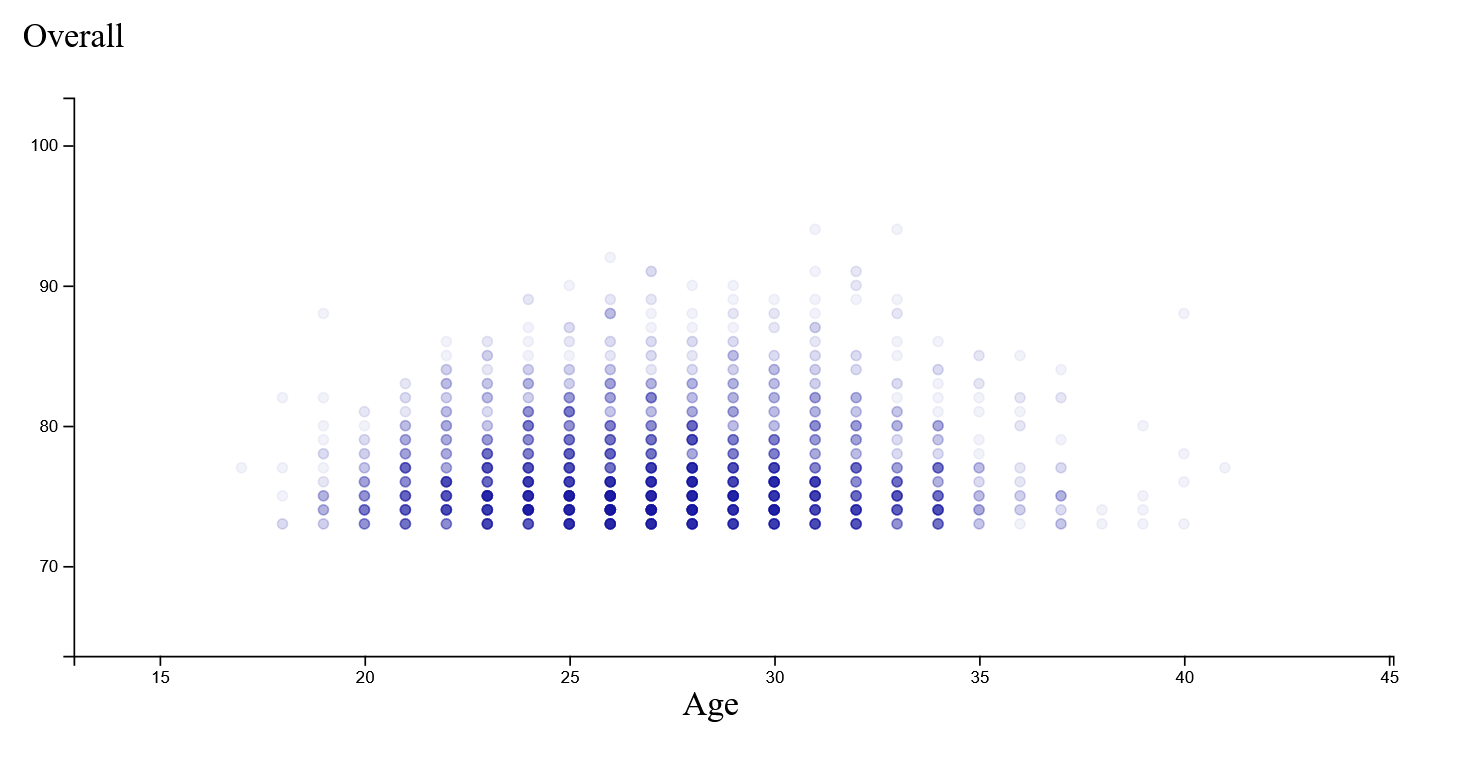
\includegraphics[scale=0.4]{grafiken/Scatterplot1}
\caption{Darstellung des Scatterplots\\ Quelle: eigene Darstellung}
\end{figure}


\subsubsection{Visualisierung Zwei}

\begin{figure}[h]
\centering
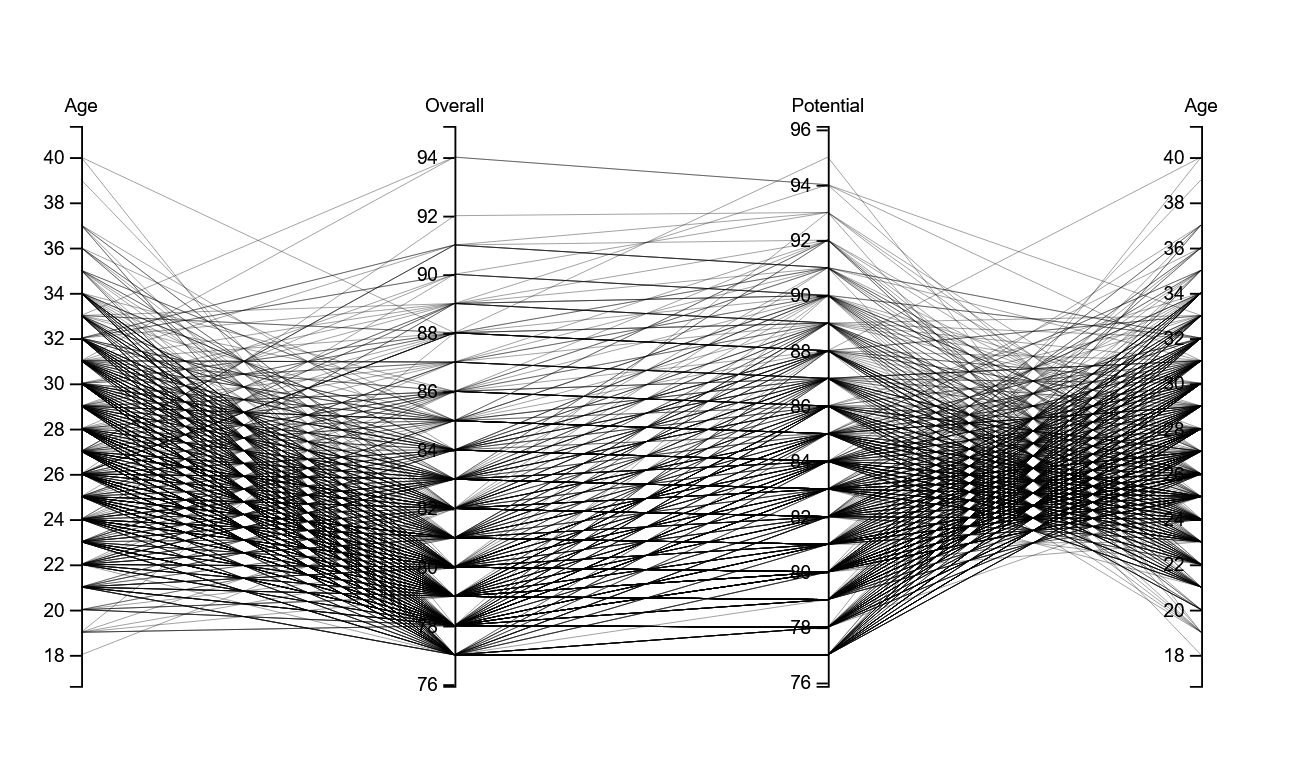
\includegraphics[scale=0.4]{grafiken/ParalleleKoordinaten1}
\caption{Darstellung der Parallelen Koordinaten\\ Quelle: Eigene Darstellung}
\end{figure}



\begin{figure}[h]
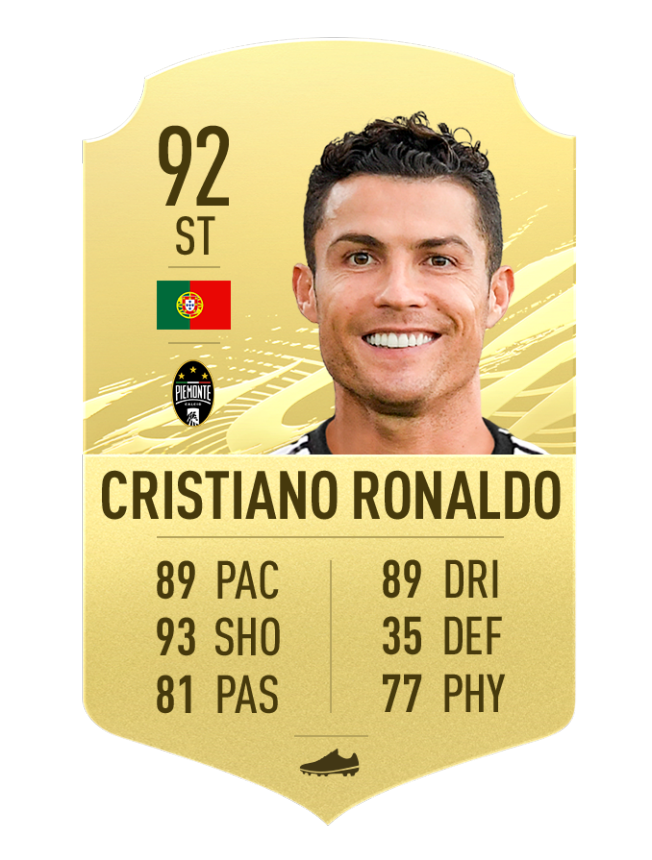
\includegraphics[scale=0.2]{grafiken/Ronaldo}
\caption{Darstellung einer FUT Karte inklusive relevanter Werte am Beispiel Cristiano Ronaldo\\ Quelle: https://www.ea.com/de-de/games/fifa/fifa-21/news/fifa-21-player-ratings-best-strikers-st-cf}
\end{figure}


\subsubsection{Visualisierung Drei}
\begin{figure}[h]
\centering
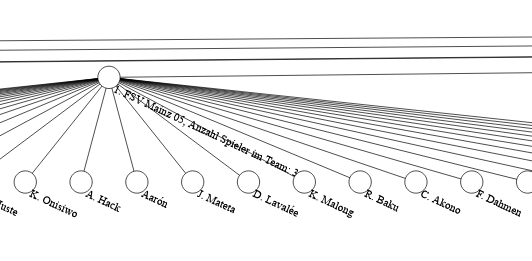
\includegraphics[scale=0.4]{grafiken/BaumDiagram1}
\caption{Ausschnitt aus Baumdarstellung\\ Quelle: Eigene Darstellung}
\end{figure}


\subsection{Interaktion}
%Erklären sie die möglichen Interaktionen mit den einzelnen Visualisierungen und die möglichen Verknüpfungen zwischen ihnen. Begründen Sie warum die konkreten Interaktionen umgesetzt wurden und welche Zwecke für die Anwenderinnen mit ihnen unterstützt werden. Begründen sie ebenfalls warum sie andere Interaktionsmöglichkeiten nicht umgesetzt haben. 

\textbf{Interaktionen in den Visualisierungen(möglicherweise Interaktion zwischen den Techniken), Warum genau diese Techniken, welche Zwecke erfüllen sie für die Anwender, Warum wurden andere nicht umgesetzt}

\section{Implementierung}
%Beschreiben Sie die Implementierung ihrer Visualisierungsanwendung in Elm. Stellen die Gliederung ihres Quellcodes vor. Haben Sie verschiedene Elm-Module erstellt. Was war aufwändig umzusetzen, was ließ sich mit dem vorhanden Code aus den Übungen relativ einfach umsetzen? 

%Wie sieht die Elm-Datenstruktur für das Model aus, in dem die verschiedenen Zustände der Interaktion gespeichert werden können.

\textbf{Wie ist der Quellcode gegliedert, was lies sich aus den Übungen übernehmen, Wie sieht die Datenstruktur des Modells aus -> in dem verschiedene Zustände der Interaktion gespeichert wurden (Success record)}

\section{Anwendungsfälle}
%Präsentieren sie für jede der drei Visualisierungen einen sinnvollen Anwendungsfall in dem ein bestimmter Fakt, ein Muster oder die Abwesenheit eines Musters visuell festgestellt wird. Begründen sie warum dieser Anwendungsfall wichtig für die Zielgruppe der Anwenderinnen ist. Diskutieren sie weiterhin, ob die oben beschriebene Information auch mit anderen Visualisierungstechniken hätte gefunden werden können. Falls dies möglich wäre, vergleichen sie die den Aufwand und die Schwierigkeiten ihres Ansatzes und der Alternativen. 

\textbf{Spezifischen Anwendungsfall für Nutzergruppen vorstellen, der an Hand der Visualisierungstechniken visuell erkennbar ist, wäre dies auch mit anderen Techniken möglich gewesen? Aufwand mit anderen Techniken vergleichen}
\subsection{Anwendung Visualisierung Eins}



\subsection{Anwendung Visualisierung Zwei}


\subsection{Anwendung Visualisierung Drei}

\section{Verwandte Arbeiten}
%Führen sie eine kurze Literatursuche in der wissenschaftlichen Literatur zu Informationsvisualisierung und Visual Analytics nach ähnlichen Anwendungen durch. Diskutieren sie mindestens zwei Artikel. Stellen sie Gemeinsamkeiten und Unterschiede dar.
\textbf{Zwei Artikel mit ähnlichen Zielen diskutieren}
\section{Zusammenfassung und Ausblick}
%Fassen sie die Beiträge ihre Visualisierungsanwendung zusammen. Wo bietet sie für die Personen der Zielgruppe einen echten Mehrwert.

\textbf{Beiträge der Anwendung, welcher Mehrwert für Zielgruppe entsteht, mögliche Erweiterungen(Visualisierungen oder Daten)}
%Was wären mögliche sinnvolle Erweiterungen, entweder auf der Ebene der Visualisierungen und/oder auf der Datenebene?

\newpage

\pagenumbering{Roman}
\setcounter{page}{4}
\section*{Anhang: Git-Historie}

\printbibliography

\end{document}

